\documentclass[12pt]{article}
\usepackage[margin=1in]{geometry}
\usepackage{setspace}
\onehalfspacing

% Start of preamble
%==========================================================================================%
% Required to support mathematical unicode
\usepackage[warnunknown, fasterrors, mathletters]{ucs}
\usepackage[utf8x]{inputenc}

\usepackage[dvipsnames,table,xcdraw]{xcolor} % colors
\usepackage{hyperref} % links
\hypersetup{
	colorlinks=true,
	linkcolor=blue,
	filecolor=magenta,      
	urlcolor=cyan,
	pdfpagemode=FullScreen
}

% Standard mathematical typesetting packages
\usepackage{amsmath,amssymb,amscd,amsthm,amsxtra, pxfonts}
\usepackage{mathtools,mathrsfs,dsfont,xparse}

% Symbol and utility packages
\usepackage{cancel, textcomp}
\usepackage[mathscr]{euscript}
\usepackage[nointegrals]{wasysym}
\usepackage{apacite}

% Extras
\usepackage{physics}  % Lots of useful shortcuts and macros
\usepackage{tikz-cd}  % For drawing commutative diagrams easily
\usepackage{microtype}  % Minature font tweaks

\usepackage{enumitem}
\usepackage{titling}

\usepackage{graphicx}
\usepackage{wrapfig}

% Fancy theorems due to @intuitively on discord
\usepackage{mdframed}
\newmdtheoremenv[
backgroundcolor=NavyBlue!30,
linewidth=2pt,
linecolor=NavyBlue,
topline=false,
bottomline=false,
rightline=false,
innertopmargin=10pt,
innerbottommargin=10pt,
innerrightmargin=10pt,
innerleftmargin=10pt,
skipabove=\baselineskip,
skipbelow=\baselineskip
]{mytheorem}{Theorem}

\newenvironment{theorem}{\begin{mytheorem}}{\end{mytheorem}}

\newmdtheoremenv[
backgroundcolor=BurntOrange!30,
linewidth=2pt,
linecolor=BurntOrange,
topline=false,
bottomline=false,
rightline=false,
innertopmargin=10pt,
innerbottommargin=10pt,
innerrightmargin=10pt,
innerleftmargin=10pt,
skipabove=\baselineskip,
skipbelow=\baselineskip
]{mycorollary}{Corollary}

\newenvironment{corollary}{\begin{mycorollary}}{\end{mycorollary}}


\newmdtheoremenv[
backgroundcolor=OrangeRed!30,
linewidth=2pt,
linecolor=OrangeRed,
topline=false,
bottomline=false,
rightline=false,
innertopmargin=10pt,
innerbottommargin=10pt,
innerrightmargin=10pt,
innerleftmargin=10pt,
skipabove=\baselineskip,
skipbelow=\baselineskip
]{mylemma}{Lemma}

\newenvironment{lemma}{\begin{mylemma}}{\end{mylemma}}

\newtheoremstyle{definitionstyle}
	{\topsep}%
	{\topsep}%
	{}%
	{}%
	{\bfseries}%
	{.}%
	{.5em}%
	{}%
\theoremstyle{definitionstyle}
\newmdtheoremenv[
backgroundcolor=Violet!30,
linewidth=2pt,
linecolor=Violet,
topline=false,
bottomline=false,
rightline=false,
innertopmargin=10pt,
innerbottommargin=10pt,
innerrightmargin=10pt,
innerleftmargin=10pt,
skipabove=\baselineskip,
skipbelow=\baselineskip,
]{mydef}{Definition}
\newenvironment{definition}{\begin{mydef}}{\end{mydef}}

\newtheorem*{remark}{Remark}

\newtheorem*{example}{Example}

% Common shortcuts
\def\mbb#1{\mathbb{#1}}
\def\mfk#1{\mathfrak{#1}}

\def\bN{\mbb{N}}
\def \C{\mbb{C}}
\def \R{\mbb{R}}
\def\bQ{\mbb{Q}}
\def\bZ{\mbb{Z}}
\def \cph{\varphi}
\renewcommand{\th}{\theta}
\def \ve{\varepsilon}
\newcommand{\mg}[1]{\| #1 \|}

% Sometimes helpful macros
\newcommand{\floor}[1]{\left\lfloor#1\right\rfloor}
\newcommand{\ceil}[1]{\left\lceil#1\right\rceil}
\renewcommand{\qed}{\hfill\qedsymbol}
\renewcommand{\H}{\mbb H}
\renewcommand{\S}{\mbb S}

% Sets
\usepackage{braket}

% End of preamble
%==========================================================================================%

% Start of commands specific to this file
%==========================================================================================%

\renewcommand{\ip}[2]{\langle #1, #2 \rangle}
\newcommand{\linf}[1]{\max_{1\leq i \leq #1}}
\newcommand{\seq}[2]{\qty(#1_#2)_{#2=1}^{\infty}}

%==========================================================================================%
% End of commands specific to this file

\title{Classifying $\overline{\C}$ Automorphisms and the Hyperbolic Plane}
\date{\today}
\author{Rohan Mukherjee}

\begin{document}

\maketitle

	\begin{abstract}
		In this paper we look at the Riemann Sphere, it's incredible equivalent forms, where they each aid intuition, classify it's automorphisms. From here we discuss the hyperbolic plane $\H^2$, and classify a large class of it's self-homeomorphisms. 
	\end{abstract}
	
	\section{Arithmetic in $\overline{\C}$}
	Before we look at the equivalent structures of the extended complex plane, we will first look at arithmetic on it. We define $\overline{\C} = \C \cup \set{\infty}$. Define the following:
	\begin{align*}
		&z + \infty = \infty \text{ for all $z \in \C$}\\
		&z \times \infty = \infty \text{ for all $z \in \C$}\\
		&\frac{z}0 = \infty \text{ and } \frac{z}{\infty} = 0 \text{ for all $z \in \C \setminus 0$}
	\end{align*}
	with $\infty \times \infty = \infty$, while $\infty - \infty$ and $0 \times \infty$ are left undefined. Similarly, let $\infty/0 = \infty$, $0/\infty = 0$, and leave $\infty/\infty$ and $0/0$ undefined. With these definitions $\overline{\C}$ does not define a field, as $\infty$ does not have an additive inverse. 
	
	\section{Topology}
	Now, we must define a topology on $\overline{\C}$. Being the 1-point compactification of $\C$. First,
	\begin{definition}
		A space $X$ is said to be locally compact at $x$ if there exists a compact subspace $C$ of $X$ that contains a neighborhood of $X$. IF $X$ is locally compact at each of its points, $X$ is said to be locally compact.
	\end{definition}
	We guide the reader to section 29 of Munkres for the proof of the following theorem:
	\begin{theorem}
		Let $X$ be a space. Then $X$ is locally compact Hausdorff if and only if there exists a space $Y$ satisfying the following conditions:
		\begin{enumerate}
			\item $X$ is a subspace of $Y$.
			\item The set $Y - X$ consists of a single point.
			\item $Y$ is a compact Hausdorff space.
		\end{enumerate}
		If $Y$ and $Y'$ are two spaces satisfying these conditions, then there is a homeomorphism of $Y$ with $Y'$ that equals the identity map on $X$.
	\end{theorem}
	
	The topology $Y$ is constructed as follows:
	\begin{align*}
		\mathcal{T} = \mathcal{T_X} \cup \set{Y - C | C \subset X \text{ compact }}
	\end{align*}
	For example, $\overline{\C} \setminus B_1(0)$ is an open subset of $\overline{\C}$. Next, we prove exercise 5 in the aforementioned section of Munkres, that is
	\begin{theorem}
		If $f: X_1 \to X_2$ is a homeomorphism of locally compact Hausdorff spaces, then $f$ extends to a homeomorphism of their one-point compactifications.
	\end{theorem}
	\begin{proof}
		Let $Y_1 = X_1 \cup \set{p},\; Y_2 = X_2 \cup \set{q}$ denote the one-point compactification of $X_1,\; X_2$ respectively. Define $\tilde{f}(x) = f(x)$ for $x \in X_1$, and $f(p) = q$. For any open set $U \subset Y_2$, if $q \not \in U$ then $\tilde{f}^{-1}(U) = f^{-1}(U)$ which is an open subset of $X_1$, and by how we defined the topology on $Y_1$, it too is an open subset of $Y_1$. If $q$ is in $U$, then $Y_2 \setminus U = C \subset X_2$ is compact. Thus $\tilde{f}^{-1}(C) = f^{-1}(C)$ is compact (since $f$ is a homeomorphism, its inverse is continuous). Thus $\tilde f^{-1}(U) = Y_1 \setminus \tilde f^{-1}(C)$ is open in $Y_1$, since it is the complement of a compact set in $X_1$. By running the exact same argument for the inverse map, we have proven the theorem.
	\end{proof}

	\section{Equivalent Forms of $\overline{\C}$}
	We have seen the homeomorphism from $\S^1 \setminus \set{N}$ to $\R$ previously on homework 4. The incredibly idea of stereographic projection works here as well. Define $f: \S^2 \setminus{(0,0,1)} \to \C$ by 
	\begin{align*}
		f(x, y, z) = \frac{x+iy}{1-z}
	\end{align*}
	\begin{wrapfigure}{r}{0.33\textwidth} %this figure will be at the right
		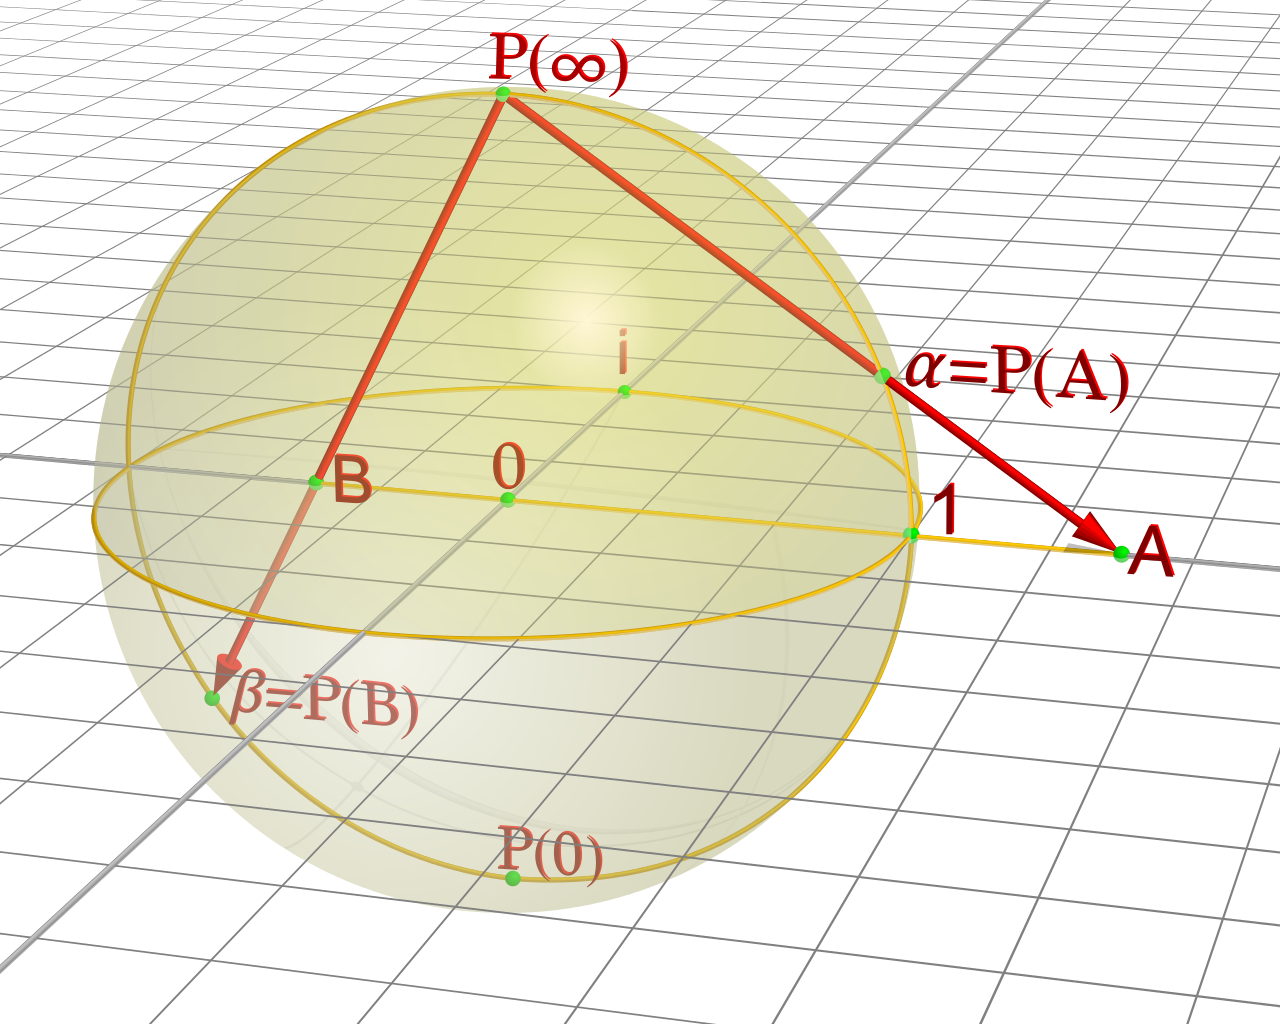
\includegraphics[width=0.33\textwidth]{projection}
	\end{wrapfigure}
	Thought of as a map from $\R^3 \to \R^2$, i.e. having $f(x, y, z) = (x/(1-z), y/(1-z))$, we see that each coordinate is a rational function in $x, y, z$, who's denominator is never 0, and thus is continuous. An equivalent formulation for this map is that if $(\theta, \cph) \in \S^2$ is the spherical coordinates for a point on the sphere, then its image will be $\cot(\frac12 \theta)e^{i\cph}$. From here, since $\cot(\frac 12 \theta)$ is surjective to $[0, \infty)$ for $\theta \in [0, \pi]$, any point $re^{i\alpha}$ will be the image of some point on the $\S^2$. Similarly, since $\cot(\frac12 \theta)$ is one-to-one and strictly positive for $\theta \in [0, \pi]$, if $\cot(\frac12 \theta_1) e^{i\cph_1} = \cot(\frac12 \theta_2) e^{i\cph_2}$, taking absolute values gives that $\theta_1 = \theta_2$, and canceling the $\cot$ from each side (unless $\theta_1 = \theta_2 = \pi$, in which case the point in question is the south pole), yields that $\cph_1 = \cph_2$, so we have guarenteed injectivity. This map also happens to have continuous inverse. Now, $\S^2$ is a compact Hausdorff space with $\S^2 \setminus \set{(0, 0, 1)} \subset \S^2$ and also $\overline{\S^2 \setminus \set{(0, 0, 1)}} = \S^2$, thus $\S^2$ is the one-point-compactification of $\S^2 \setminus \set{(0, 0, 1)}$. 
	\begin{wrapfigure}{r}{0.25\textwidth} %this figure will be at the right
		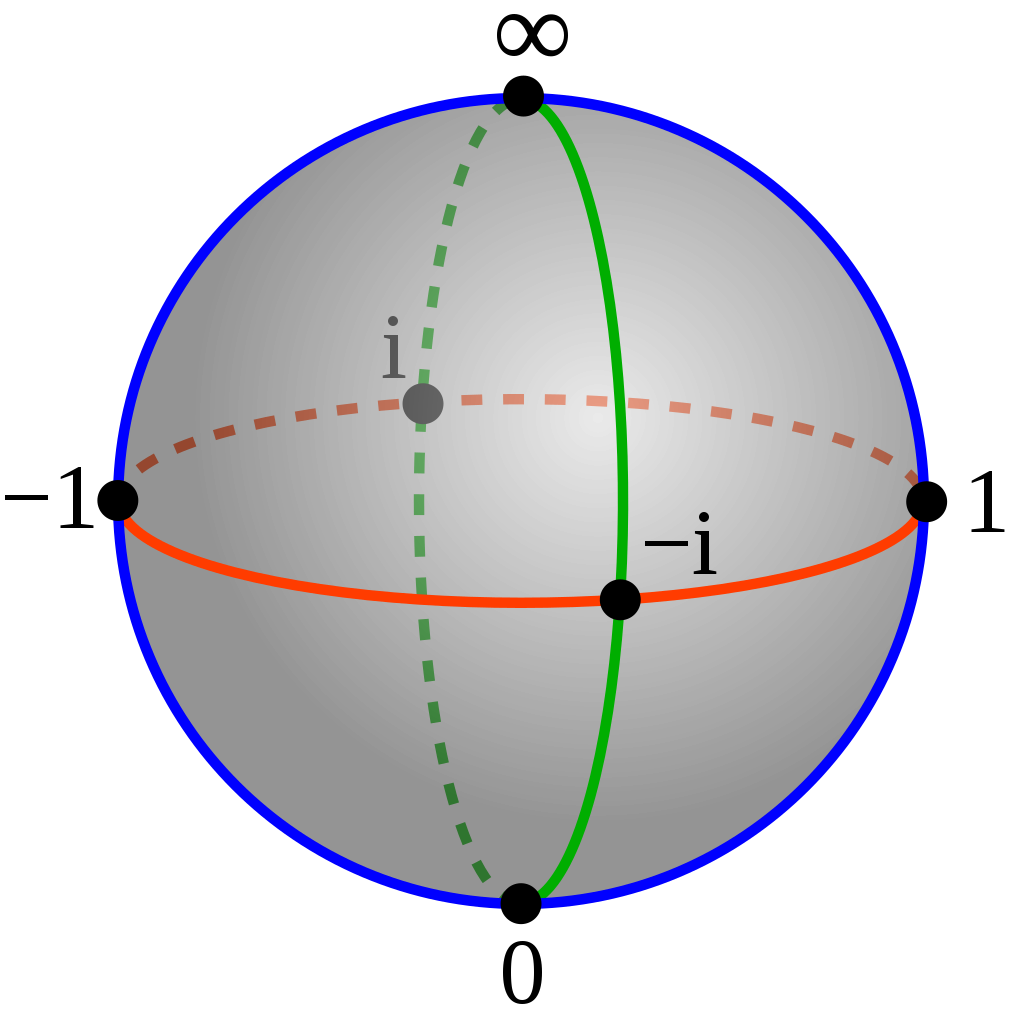
\includegraphics[width=0.25\textwidth]{riemannsphere}
	\end{wrapfigure}
	As we defined $\overline{\C}$ to be the one-point-compactification of $\C$, using the previous theorem lets us extend this homeomorphism to a homeomorphism of the sphere with the extended complex plane. For this reason the extended complex plane is sometimes called the Riemann sphere.
	
	This form is especially important for visualizing the extended complex plane. For example, since $\S^2$ is sequentially compact, every sequence has a convergent subsequence. We propose a question to the reader: what is a convergent subsequence of $(n)_{n \in \bN} \subset \overline{\C}$? Itself! $(n)_{n \in \bN} \to \infty$, which may be visualized as wrapping along the right side of the Riemann sphere.
	
	
	Now we will get to the form that will help us the most during this paper. We have seen real projective space $\R \mbb P$ before. It turns out that the extended complex plane is also homeomorphic to the complex projective space. We give the following definition:
	\begin{definition}
		We define $\C \mbb P = \bigg(\C^2 \setminus (0, 0)\bigg) \; \bigg/ \sim$ where $(z, w) \sim (\lambda z, \lambda w)$ for every $\lambda \in \C \setminus 0$.
	\end{definition}
	The topology on this space is of course the quotient topology. Showing that this is homeomorphic to $\overline{\C}$ goes as follows:
	Define the map $q: \C^2 \setminus \set{0} \to \overline{\C}$ by $q(z, v) = z/v$. We refer the reader to the MSE post in the bibliography to see the proof that this map is open and continuous (https://math.stackexchange.com/questions/410929/why-is-the-complex-projective-line-homeomorphic-to-a-2-sphere). We must now show that this map is constant on the equivalence classes. $[z, w] = \set{(\lambda z, \lambda w) | \lambda \in \C}$, thus this claim follows immediately since $\lambda z / \lambda w = z/w$. We thus have the following commutative diagram:
	\[\begin{tikzcd}
		{\C^2 - (0, 0)} \\
		\\
		{\C \mbb P} && {\overline{\C}}
		\arrow["\pi", from=1-1, to=3-1]
		\arrow["q"', from=1-1, to=3-3]
		\arrow["{\tilde{q}}", from=3-1, to=3-3]
	\end{tikzcd}\]
	where $\tilde q$ is a quotient map since we just verified that $q$ is. We need to check injectivity. If nothing is 0, $z_1/w_1 = z_2/w_2$, then $z_1/z_2 = w_1/w_2$. This says precisely that $(z_1, w_1) \in [z_2, w_2]$, hence we are done. if $w_1 = 0$, then $w_2$ is necessarily 0 (note that $z_2 \in \C$, not $\overline{\C}$). Thus they are in the same equivalence class. If $z_1 = 0$, then $z_2 = 0$ by the same reasoning. Symmetry covers the rest of the cases, thus we have checked injectivity. A bijective quotient map is a homeomorphism, thus we are done. This form of the extended complex plane will be especially helpful--via this homeomorphism, any rational function translates immediately into a continuous function on the complex projective plane by $f/g \leftrightarrow [f(x), g(x)]$.
	
	\section{Automorphisms of $\overline{\C}$}
	For all our purposes, an automorphism from $\overline{\C}$ to $\overline{\C}$ is a bijective holomorphic function (this automatically guarentees holomorphic inverse). Holomorphic in this case just means $C^\infty$, we refer the reader to Stein \& Shakarchi Book 2 for reference. We introduce the holy grail of all holomorphic maps, so important that they are given a special name: conformal mappings AKA Möbius transformations, maps of the form
	\begin{align*}
		f(z) = \frac{az+b}{cz+d}, \; a, b, c, d \in \C \text{ with } ad -  bc \neq 0
	\end{align*}
	The condition $ad-bc \neq 0$ should be familiar to the reader--it is equivalent to the determinant of the matrix $\begin{pmatrix}
		a & b \\ c & d
	\end{pmatrix}$ having nonzero determinant. Recall from the previous section that the rational function $f$ can be expressed as $[az+b, cz+d]$ in projective coordinates, which may be rewritten as $[z, 1] \cdot \begin{pmatrix} a & b \\ c & d \end{pmatrix}$. Now the condition shouldn't come as such a surprise! Long, tedious calculations show that composing Möbius transformations is the exact same as composing these matrices--in particular, the composition of two Möbius transformations is another Möbius transformation. Also, given $ad-bc \neq 0$, the inverse Möbius transformation would be 
	\begin{align*}
		f^{-1}(z) = \frac{dz-b}{-cz+a}
	\end{align*}
	which should not come as a surprise. 
	One can extend a function $f: \C \to \C$ to include $\infty$ in it's domain by defining $f(\infty) = \lim_{z \to \infty} f(\infty)$ when the limit exists. $f$ is necessarily continuous at $\infty$ as given any $w_n \to \infty$, $\lim_{n \to \infty} f(w_n) = \lim_{z \to \infty} f(z) = f(\infty)$ (We may use this equivalent form of continuity since $\overline \C$ is first-countable, being homeomorphic to $\S^2$.) $f$ is said to be meromorphic at $\infty$ if $f(1/z)$ is meromorphic in $0$. We may also include $\infty$ in the range: if $f(z)^{-1}$ has a zero at $a \in \overline{\C}$, then we say that $f(a) = \infty$. One calls $f$ meromorphic if it is meromorphic at each $a \in \overline \C$. I claim that meromorphic implies continuity. Indeed, letting $a \in \overline \C$ be arbitrary, if $a \neq \infty$, and $f(a) \neq \infty$, then $f(a)$ is analytic (as a complex function) and hence obviously continuous. If $f(a) = \infty$, $f(z)^{-1}$ has a 0 at $a$, and is analytic there (by definition of a pole), so is continuous. Finally, for any $M \in \bN$, we need to find a neighborhood $U = \overline \C \setminus K$ ($K$ compact) of $\infty$ so that $|f(z)| \geq M$ for every $z \in U$. This follows directly from the definition of $f(\infty)$.
	Now, we note the following incredibly surprising fact:
	\begin{theorem}
		If $f: \overline{\C} \to \overline{\C}$ is an automorphism (bijective meromorphic function), then $f$ is a Möbius transformation of the form $\frac{az+b}{cz+d}$ with $ad-bc \neq 0$.
	\end{theorem}
	This theorem is laughably false for real-valued functions. For example, $x^n$ for any odd $n$ is an automorphism of $\R$. The proof is very long and very hard, so we will just prove this lemma:
	\begin{lemma}
		If $f: \C \to \C$ is holomorphic everywhere, and injective, then it is of the form $f(z) = az + b$ with $a \neq 0$.
	\end{lemma}
	This lemma depends on something  called the Casorati-Weirstrass theorem and the open mapping theorem, which we will use but not provide here. 
	\begin{proof}
		We write $f(z) = \sum_{n=0}^\infty a_nz^n$. We have two cases: the sum has finitely many terms, or it doesn't. In the second case, since $f(1/z)$ is holomorphic in $\C \setminus 0$, and has an essential singularity in 0, $f(B_1(0) \setminus 0)$ is dense in $\C$. Consider any point $w \in f(\C \setminus \overline{B_1(0)})$. Find $\ve > 0$ so that $B_\ve(w) \subset f(\C \setminus \overline{B_1(0)})$, which we can do since $f$ is an open map by the open mapping theorem. By density, find a $z \in B_1(0) \setminus 0$ so that $f(z) \in B_\ve(w)$. But since $B_1(0)$ and $\C \setminus \overline{B_1(0)}$ are disjoint open sets, their image is also disjoint and open (by injectivity), which this immediately contradicts. So $f(z) = \sum_{n=0}^m a_nz^n$. Suppose that there was some $a_n \neq 0$ for some $n > 1$. Then $f$ would be a degree $m$ polynomial with $m > 1$. Thus factor $f(z) = \prod_{i=0}^m (z_i-\alpha_i)$. If $\alpha_i$ is always the same, $f(z) = 1$ would have $m > 1$ solutions, a contradiction. Else, $f$ has at least two distinct roots, another contradiction. Thus $f(z) = az + b$. Constants are not injective, so $a \neq 0$, and we are done.
	\end{proof}
	We have seen the geometric side of things. Now, let's look at the algebraic side of things.
	
	\section{Algebra}
	Now define \begin{align*}
		\mathrm{Aut}(\overline \C) = \Set{\frac{az+b}{cz+d} | a,b,c,d \in \C, \; ad-bc \neq 0}
	\end{align*}
	Let $\mathrm{GL_2}(\C)$ denote the group of 2 $\times$ 2 matrices who have nonzero determinant. A quick calculation shows that matrix multiplication and composition of mobius transformations are precisely the same, so we can define a group homomorphism \begin{align*}
		\cph: \begin{pmatrix}
			a & b\\ c & d
		\end{pmatrix}
		\mapsto \frac{az+b}{cz+d}
	\end{align*}
	from $\mathrm{GL_2}(\C)$ to $\mathrm{Aut}(\overline \C)$. The identity automorphism is of course $f(z) = z$. Thus $\ker(\cph)$ consists of the matrices $\begin{pmatrix}
		a & b\\ c & d
	\end{pmatrix}$ so that $\frac{az+b}{cz+d} = z$ for all $z$, and it is not hard to see that this happens iff $a = c \neq 0$, $c = d = 0$. Thus the kernel is precisely
	\begin{align*}
		\ker(\cph) = \Set{\begin{pmatrix}
				\lambda & 0 \\ 0 & \lambda
			\end{pmatrix}
			| \lambda \in \C - 0}
	\end{align*}
	We define $\mathrm{PGL}_2(\C)$ as the quotient $\mathrm{GL}_2(\C) \bigg / \ker(\cph)$ (relating to a group of matrices acting on $\C \mbb P$, which is also the extended complex plane!), and by the above theorem this map is onto, hence \begin{theorem}
		$\mathrm{Aut}(\overline \C) \cong \mathrm{GL}_2(\C) \bigg / \ker(\cph) = \mathrm{PGL}_2(\C)$.
	\end{theorem}. By the above we also now have a good intuition for the a group acting on $\C \mbb P \cong \overline{\C} \cong \S^2$. So, what does this mean? matrices tell you how you stretch and rotate the unit square. By modding out by $\ker(\cph)$, we may multiply by the matrix $\begin{pmatrix}
		\sqrt{1/\det(M)} & 0 \\ 0 & 1/\sqrt{\det(M)}
	\end{pmatrix}$, who's determinant is $1/\det(M)$, and represent each element of this quotient group by a matrix with determinant 1. Geometrically this means we are no longer stretching, just rotating. That is indeed the next result:
	\begin{theorem}
		Recall that $\mathrm{SL}_2(\C) = \Set{\begin{pmatrix}
				a & b \\ c & d
			\end{pmatrix} | a, b, c, d \in \C, \; ad-bc = 1}$. Write $\mathrm{PSL}_2(\C) = \pi(\mathrm{SL}_2(\C))$, where $\pi$ is the projection from $\mathrm{GL_2}(\C)$ to $\mathrm{GL}_2(\C) \bigg / \ker(\cph)$. Then $\mathrm{Aut}(\overline \C) \cong \mathrm{PGL}_2(\C) = \mathrm{PSL}_2(\C)$.
	\end{theorem}
	We define
	\begin{definition}
		A circle in the sphere $\S^2 \subset \R^3$ is the intersection $\S^2 \cap \Pi$ where $\Pi$ is a plane in $\R^3$ that is intersecting and not tangent to $\S^2$. A circle in $\overline \C$ is thus the image of this set under the prescribed homeomorphism.
	\end{definition}
	A long calculation shows that if $\alpha x_1 + \beta x_2 + \gamma x_3 = \delta$ ($\alpha, \beta, \gamma \in \R$) is a plane corresponding to the circle $C$ in $\S^2$, then $C$ is given by the equation $2\alpha \Re(z) + 2 \beta \Im(z) + \gamma(|z|^2-1) = \delta(|z|^2+1)$. Referencing the book, this leads to there being two types of circles: regular circles in $\C$, and straight lines in $\C$ along with $\infty$ (which, on the Riemann sphere, is of course still a circle). Finally,
	\begin{theorem}
		If $C$ is a circle of $\overline \C$, and if $T \in \mathrm{PGL_2}(\C)$, then $T(C)$ is a circle of $\overline \C$.
	\end{theorem}
	But first,
	\begin{lemma}
		Every mobius transformation is the composition of
		\begin{enumerate}[label=(\roman*)]
			\item Transformations of the form $e^{i\theta} z$ ($\theta \in \R$), representing a rotation of the sphere $\S^2$ by an angle $\theta$ about the vertical axis,
			\item The transformation $z \mapsto z^{-1}$, representing a horizontal rotation by $\pi$,
			\item The transformations $z \mapsto rz$, $r \in \R_{>0}$ (stretching),
			\item The transformations $z \mapsto z + t$, $(t \in \C)$ (translations).
		\end{enumerate}
	\end{lemma}
	\begin{proof}
		By the above isomorphism, every mobius transformation is of the form $T(z) = (az+b)/(cz+d)$ with $ad-bc = 1$. If $c = 0$ then $T(z) = (az+b)/d$ with $a, d \neq 0$ so let $a/d = re^{i\theta}$ and $b/d = t$. Then $T(z) = re^{i\theta} + t$, so
		\[\begin{tikzcd}
			{\overline \C} && {\overline \C} && {\overline \C} && {\overline \C}
			\arrow["{z \mapsto e^{i\theta}z}", from=1-1, to=1-3]
			\arrow["{z \mapsto rz}", from=1-3, to=1-5]
			\arrow["{z \mapsto z + t}", from=1-5, to=1-7]
			\arrow["T"', bend left, from=1-1, to=1-7]
		\end{tikzcd}\]
	\end{proof}
	\begin{proof}[Proof (Of theorem)]
		For euclidean circles:
		\begin{enumerate}[label=(\roman*)]
			\item For circles of the form $(x-a)^2 + (y-b)^2 = R^2$, one sees that the map $x+iy \mapsto x\cos(\theta)-y\sin(\theta)+i(x\sin(\theta)+y\cos(\theta))$ yields
			\begin{align*}
				(x\cos(\theta)-y\sin(\theta)-a)^2 + (x\sin(\theta)+y\cos(\theta)-b)^2 &= R^2 \iff \\
				x^2-x2(a\cos(\theta)+b\sin(\theta)) + b^2 + y^2 +y2(a\sin(\theta)-b\cos(\theta)) + a^2 &= R^2
			\end{align*}
			Now, from the identity $(a \cos(\theta)+b \sin(\theta))^2+(a\sin(\theta)-b\cos(\theta))^2 = a^2+b^2$, we see we do not need to add anything to complete the square, and thus our circle is
			\begin{align*}
				(x-(a\cos(\theta)+b\sin(\theta))^2 + (y+(a\sin(\theta)-b\cos(\theta)) = R^2
			\end{align*}
			This is of course what we expected, as the center $(a, b)$ under the aforementioned transformation gets mapped there. Similarly, \item For $z \mapsto rz$, we would get 
			\begin{align*}
				(rx-a)^2 + (ry-b)^2 &= R^2 \iff \\
				(x-a/r)^2 + (y-b/r)^2 &= (R/r)^2
			\end{align*}
			\item The final translation $z \mapsto z+(c+id)$ is clear and done in a similar fashion.
		\end{enumerate}
		For circles of the form $\Lambda \cup \infty$ where $\Lambda$ is a straight line in $\C$, the default equation is $y = mx + b$. Thus,
		\begin{enumerate}[label=(\roman*)]
			\item The transformation $x+iy \mapsto x\cos(\theta)-y\sin(\theta)+i(x\sin(\theta)+y\cos(\theta))$ gives
			\begin{align*}
				x\sin(\theta)+y\cos(\theta) = m(x\cos(\theta)-y\sin(\theta)) + b \\
				x(\sin(\theta)-m\cos(\theta)) + y(\cos(\theta)+m\sin(\theta)) = b
			\end{align*}
			Which is clearly seen to be a line. Next,
			\item The transformation $x+iy \mapsto rx + iry$ yields
			\begin{align*}
				ry = mrx + b \iff y = mx + b/r
			\end{align*}
			Again clearly a line. Finally,
			\item The translation $x + iy \mapsto x + iy + (c+id)$ is clear like last time. 
		\end{enumerate}
	
		By the lemma every Mobius transformation is a composition of (at most three) of these. Since each of these maps circles to circles, the theorem has been proved.
	\end{proof}
	Finally,
	\begin{theorem}
		The map $z \mapsto \overline{z}$ is a circle-preserving homeomorphism.
	\end{theorem}
	This theorem can be proved in the same exact way as before, and is therefore left as an exercise to the reader.
	
	\section{The reverse implication}
	\begin{theorem}
		If $f$ is a circle preserving homeomorphism of $\overline \C$, then $f$ is a Mobius transformation or the composition of complex conjugate with a Mobius transformation.
	\end{theorem}
	Now this is quite the spectacular theorem. This gives rise to a very large class of homeomorphisms of $\overline \C$, which is topologically important, and has huge applications to hyperbolic geometry, which we will not discuss. First,
	\begin{lemma}
		If $X \subset \overline \C$ is dense, and $f: \overline \C \to \overline \C$ is a continuous function so that $f(z) = z$ for all $z \in X$, then $f$ is the identity.
	\end{lemma}
	\begin{proof}
		Sequential continuity is equivalent to regular continuity for first-countably spaces. It follows then that for any $z \in \overline \C$, there is some $(z_n) \to z$ with each $z_n \in X$. Now, 
		% https://q.uiver.app/#q=WzAsNCxbMCwwLCJmKHpfbikiXSxbMiwwLCJmKHopIl0sWzAsMSwiel9uIl0sWzIsMSwieiJdLFswLDFdLFswLDIsIj0iLDMseyJzdHlsZSI6eyJib2R5Ijp7Im5hbWUiOiJub25lIn0sImhlYWQiOnsibmFtZSI6Im5vbmUifX19XSxbMSwzLCI9IiwzLHsic3R5bGUiOnsiYm9keSI6eyJuYW1lIjoibm9uZSJ9LCJoZWFkIjp7Im5hbWUiOiJub25lIn19fV0sWzIsM11d
		\[\begin{tikzcd}
			{f(z_n)} && {f(z)} \\
			{z_n} && z
			\arrow[from=1-1, to=1-3]
			\arrow["{=}"{marking}, draw=none, from=1-1, to=2-1]
			\arrow["{=}"{marking}, draw=none, from=1-3, to=2-3]
			\arrow[from=2-1, to=2-3]
		\end{tikzcd}\]
	\end{proof}
	\begin{theorem}
		If $m(z)$ fixes three distinct points of $\overline \C$, then $m(z)$ is the identity.
	\end{theorem}
	\begin{proof}
		If $m(\infty) = \infty$, then $c = 0$. This yields $m(z) = az + b$ for some $a,  b$. Fixing two points means that the linear polynomial $(a-1)z + b = 0$ has two solutions, which can only happen if $a = 1$ and $b = 0$. Similarly, if $c \neq 0$, then $m(\infty) \neq \infty$. So all three fixed points lie in $\C$. Notice that 
		\begin{align*}
			\frac{az+b}{cz+d} = z \iff az+b = cz^2 + dz \iff cz^2 + z(d-a) - b = 0
		\end{align*}
		is a quadratic. To have three roots, this quadratic must be equivalently 0, that is, $c = 0$, $d = a$, and $b = 0$, which is again the identity.
	\end{proof}
	\begin{theorem}
		There is a unique Mobius transformation sending $(z_1, z_2, z_3)$ to $(w_1, w_2, w_3)$.
	\end{theorem}
	\begin{proof}
		(Uniqueness) Let $m$ and $n$ be Mobius transformations doing the above. Then $n^{-1} m$ is a Mobius transformation fixing three points and hence is the identity.
		
		
		(Existence)
		When all the $z_1, z_2, z_3$ lie in $\C$, the map
		\begin{align*}
			m(z) = \frac{z-z_1}{z-Z_3} \frac{z_2-z_3}{z_2-z_1} = \frac{(z_2-z_3)z - z_1(z_2-z_3)}{(z_2-z_1)z - z_3(z_2-z_1)}
		\end{align*}
		sends $(z_1, z_2, z_3)$ to $(0, 1, \infty)$ by plugging things in, and is Mobius since $ad-bc = (z_2-z_3)(-z_3)(z_2-z_1) - (-z_1)(z_2-z_3)(z_2-z_1) = (z_2-z_3)(z_1-z_3)(z_2-z_1)$ which is nonzero since the $z_i$'s are distinct. For the map sending $(\infty, z_2, z_3)$ to $(0, 1, \infty)$, the function
		\begin{align*}
			m(z) = \frac{z_2-z_3}{z-z_3}
		\end{align*}
		works. The case $\infty \mapsto \infty$ results in picking $c = 0$, and is so simple I leave it as an exercise to the reader. Now, let $m$ be the map sending $(z_1, z_2, z_3)$ to $(0, 1, \infty)$, and let $n$ be the map sending $(w_1, w_2, w_3)$ to $(0, 1, \infty)$. The map $n^{-1} m$ is the desired map, and the theorem has been proved.
	\end{proof}
	I reference the book in that three distinct points in $\overline \C$ uniquely identify a circle (or a line, if one of the points is $\infty$). 
	
	\begin{proof}[Proof (Of theorem).]
		We now give the proof of the aforementioned theorem in all it's glory. We have already seen that all of those maps are circle-preserving homeomorphisms. We must prove the other direction. Let $f$ be a circle-preserving homeomorphism, and let $p$ be the Mobius transformation sending $(f(0), f(1), f(\infty))$ to $(0, 1, \infty)$, so $p \circ f$ satisfies $p \circ f(0) = 0$, $p \circ f(1) = 1$, and $p \circ f(\infty) = \infty$. $\overline \R$ (the extended real line) is the unique circle determined by $(0, 1, \infty)$, and thus $f(\overline \R) = \overline \R$.
		
	 	I claim that $p \circ f (\mbb H)$ is either the upper-half or the lower-half plane. Notice that nothing in this image can lie on the extended real line by bijectivity. Case 1: there is some $z \in \mbb H$ so that $p \circ f (z) \in \mbb H$. Now suppose that there was some $w \in \mbb H$ so that $p \circ f(w)$ had negative real part. Letting $\Lambda$ be the straight line connecting $z$ to $w$, $\Lambda$ is connected while $(p \circ f(\Lambda) \cap \mbb H, p \circ f(\Lambda) \cap -\mbb H)$ forms a disconnection of the image, a contradiction. Suppose, with the previous conditions still holding, there was some $a \in - \mbb H$ so that $p \circ f(a)$ had positive real part. The segment connecting $f(z)$ to $f(a)$ is connected but it's preimage is not, which contradicts $p \circ f$ being a homeomorphism. This shows that $f(\overline \H) = \overline \H$ in this case. The other case is extremely similar and is left as an exercise to the reader, so the only other possibility is that $f(\overline \H) = -\mbb \H)$. 
		
		In the first case set $m = p$, and in the second set $m = C \circ p$, where $C$ is complex conjugation. This yields a map preserving the upper half plane, and sending $(0, 1, \infty)$ to itself. Let $Z$ denote the set of fixed points of $m \circ f$. Notice that $\set{0, 1, \infty} \subset Z$. Since $m \circ f$ fixes $\infty$, if $m \circ f$ sends Euclidean lines in $\C$ (regular lines) to Euclidean lines in $\C$, and Euclidean circles in $\C$ to Euclidean circles in $\C$. I claim that if $X, Y$ are two Euclidean circles in $\C$ that intersect at $z_0$, with $m \circ f(X) = X$ and $m \circ f(Y) = Y$, then $m \circ f(z_0) = z_0$. This follows since $f(z_0) \in X \cap Y$, which has a unique intersection point, so $z_0$ is in $Z$ in this case. 
		
		For each $s \in \R$, let $V(s)$ be the vertical line in $\C$ through $s$ and let $H(s)$ be the vertical line in $\C$ through $is$.
		
		Let $H$ be any horizontal line in $\C$ that is not $\R$. As $m \circ f(\R) = \R$ and $H, \R$ are disjoint, $m \circ f(H)$ and $m \circ f(\R) = \R$ are disjoint lines in $\C$, so $H$ is a horizontal line $\C$. As $m \circ f(\H) = \H$, $H$ lies in $\H$ iff $m \circ f(H)$ lies in $\H$.
		
		Let $A$ denote the Euclidean circle with Euclidean center 1/2 and radius 1/2. As $V(0)$ is tangent (in the geometrical sense) to $A$ at 0, we see that $m \circ f(V(0))$ is tangent to $m \circ f(A)$ at $m \circ f(0) = 0$, since $m \circ f(A \cap V(0)) = (m \circ f(A)) \cap (m \circ f(V(0))$ by injectivity. Similarly $m \circ f(V(1))$ is the tangent line to $m \circ f(A)$ at 1.
		
		As $V(0)$ and $V(1)$ are parallel lines in $\C$, $m \circ f(V(0))$ and $m \circ f(V(1))$ are also parallel lines in $\C$ (by the same injectivity argument), and by rotational symmetry of the complex plane, our arguments showing that if $H$ is horizontal then $H$ lies in $\mbb H$ iff $m \circ f(H)$ lies in $\mbb H$, we can conclude that if $V$ is vertical, then $V$ lies in the right half of the complex plane iff $m \circ f(V)$ lies in the right half of the complex plane. Necessarily then $m \circ f(V(1))$ is a vertical line going through 1 and is hence $V(1)$, and by parallel $m \circ f(V(0)) = V(0)$.
		
		This forces $f(A) = A$, as the tangent lines through 0 and 1 of any other Euclidean circle passing through 0 and 1 are not parallel. One may see this by seeing that if $(x-a)^2+(y-b)^2 = r^2$, and 0 and 1 lie on this circle, then $a^2 + b^2 = r^2$, and $(1-a)^2 + b^2 = r^2$, yielding $a^2 - (1-a)^2 = 0$, which says that $a=1/2$. An explicit calculation shows that $r \geq 1$, and that if $r > 1$ the above claim holds. Even though $m \circ f(A) = A$, we do not know that $A$ contains any points of $Z$ other than 0 and 1.
		
		So we run the same argument with the two horizontal tangent lines to $A$. Considering the first tangent $H(1/2)$ to $A$ at $1/2 + 1/2 i$, we see that $m \circ f(H(1/2))$ is again a horizontal line in $\H$ tangent to $m \circ f(A)$, and so $m \circ f(H(1/2)) = H(1/2)$ ($A$ has only one tangent line that is horizontal in the upper half plane). This gives more points in $Z$, such as the intersection of the above horizontal and vertical lines, i.e. the points $1/2i$ and $1 + 1/2 i$. Running the same argument on $H(-1/2)$ yields that the points $-1/2i$ and $1 - 1/2i$ lie in $Z$. 
		
		\newpage
		
		By running this exact same argument on the circle centered at $x > 0$ with radius $x$, we get that the entire imaginary axis is in $Z$, and the line segments starting from $(1/2, 0)$ with slope of 1, and starting from $(1/2, 0)$ with slope of -1. 
		
		
		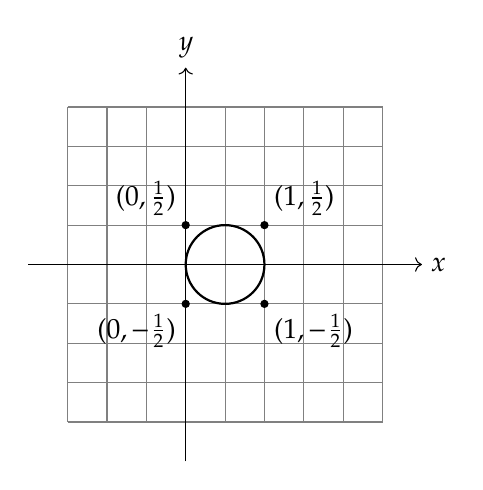
\begin{tikzpicture}
			
			\draw[step=0.5,gray,thin] (-1.5,-2) grid (2.5,2);
			\draw[->] (-2,0) -- (3,0) node[right] {$x$};
			\draw[->] (0,-2.5) -- (0,2.5) node[above] {$y$};
			
			% Draw the circle
			\draw[thick] (1/2, 0) circle [radius=1/2];
			
			% Label the points
			\fill (0,1/2) circle [radius=1.5pt] node[above left] {$(0,\frac{1}{2})$};
			\fill (1,1/2) circle [radius=1.5pt] node[above right] {$(1,\frac{1}{2})$};
			\fill (1,-1/2) circle [radius=1.5pt] node[below right] {$(1,-\frac{1}{2})$};
			\fill (0, -1/2) circle [radius=1.5pt] node[below left] {$(0,-\frac{1}{2})$};
			
		\end{tikzpicture}
		$\quad \quad \quad \quad \quad \quad \quad \quad \quad$
		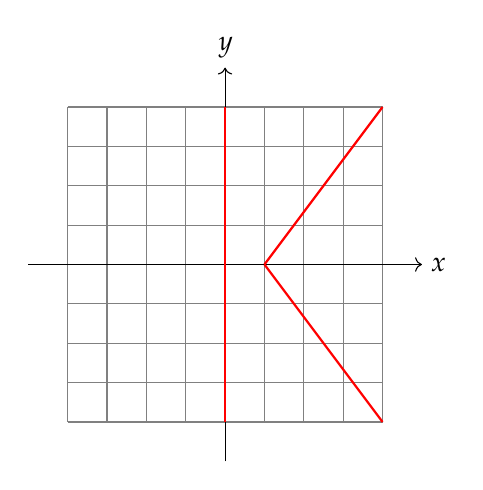
\begin{tikzpicture}
			\draw[step=0.5,gray,thin] (-2,-2) grid (2,2);
			\draw[->] (-2.5,0) -- (2.5,0) node[right] {$x$};
			\draw[->] (0,-2.5) -- (0,2.5) node[above] {$y$};
			
			% Line segments
			\draw[thick, red] (1/2,0) -- (2,2);
			\draw[thick, red] (1/2,0) -- (2,-2);
			\draw[thick, red] (0, -2) -- (0, 2);
		\end{tikzpicture}
		
		
		One sees that given any two points in $Z$, the line segment connecting them is also in $Z$, since two points uniquely determine a line. For any $x > 0$, since $(0, x)$ and $(1/2 + x, x)$ are in $Z$, the horizontal line segment connecting them is as well. Similarly, for $x < 0$ the line segment connecting $(0, x)$ and $(1/2 + x, -x)$ lies in $Z$. By also getting $0$ and $1/2$ by continuity, this yields all the points in $\C$, thus $m \circ f$ is the identity map when restricted to $\C$, and hence also the identity map on $\overline \C$ by continuity. Then $f = m^{-1}$ is a Mobius transformation, or the composition of a Mobius transformation with complex conjugation, which concludes the proof of the theorem, and my paper.
	\end{proof}

\bibliographystyle{apacite}
\bibliography{citation}
\end{document}
